\documentclass[../file.tex]{subfiles}
\usepackage{graphics}

\begin{document}
	
L'architecture que nous avons imaginé n'ayant pas réellement commencé, nous n'avons pour le moment 
rien changé. Il nous faut trouver le moyen de configurer un routeur pour les machines virtuelles en les connectant 
entre elles à travers les hyperviseurs de manière transparente.

\begin{figure}[h]
    \centering
    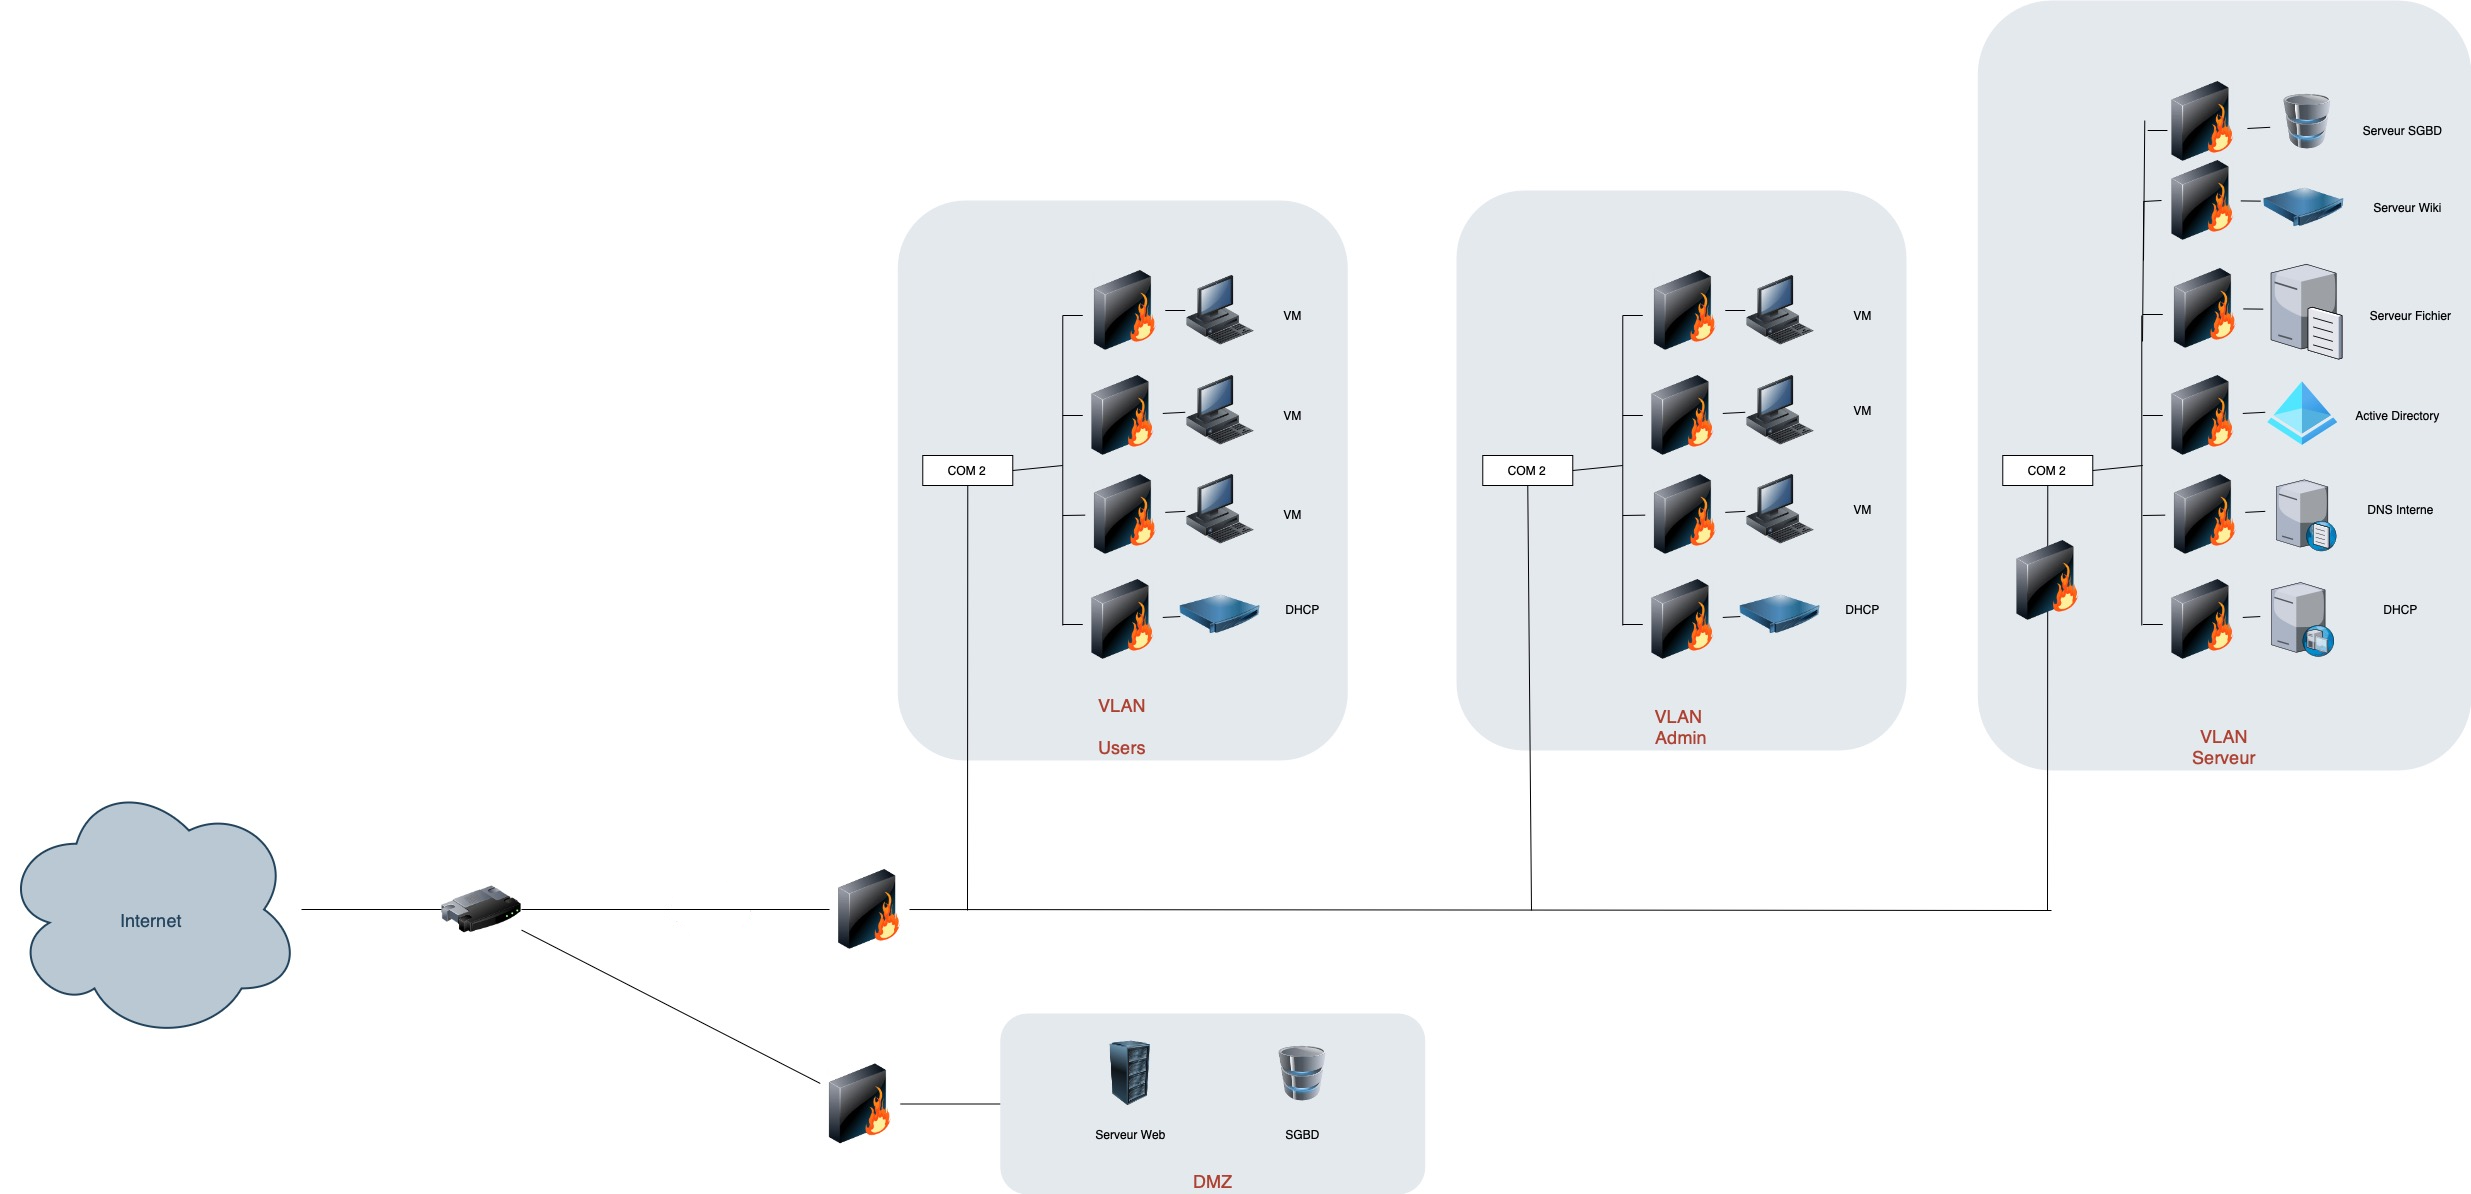
\includegraphics[width=1\textwidth]{../Images/Architecture.png}
    \caption{Architecture de la première partie}
    \label{fig:solution1}
\end{figure}

Nous avons fait pour le moment qu'une seule modification en la personne des routeurs. Nous n'avons désormais qu'un 
seul routeur qui permet d'interconnecter les réseaux qui ici sont des vlans, étant donné que nous avons un serveur DHCP 
par vlan celui ci devra rediriger les requêtes DHCP des machines vers le serveur en question et reciproquement.
Il y aura également un service DNS tourant dans la DMZ pour assurer la résolutution de nom. Donc deux serveurs DNS, 
avec celui qui se trouve dans l'intranet des serveurs

\end{document}